\documentclass[tikz,border=5mm]{standalone}
\usepackage[T1]{fontenc}
\usepackage{lmodern}
\usepackage{amsmath,amssymb}
\usepackage{xcolor}
\usepackage{tikz}
\usetikzlibrary{arrows.meta,positioning,calc,fit,backgrounds,decorations.pathreplacing,shapes.geometric}
\definecolor{regCalm}{HTML}{4C78A8}
\definecolor{regSpike}{HTML}{F58518}
\definecolor{leafgreen}{HTML}{54A24B}
\tikzset{
  treenode/.style = {rectangle, draw=black!60, fill=white, rounded corners=2pt,
                     minimum width=0.7cm, minimum height=0.45cm, inner sep=2pt,
                     font=\sffamily\fontsize{7}{8.5}\selectfont, align=center},
  activelaw/.style = {rectangle, draw=#1!80!black, fill=#1!8, rounded corners=3pt,
                      minimum width=2.0cm, minimum height=0.5cm, inner sep=3pt,
                      font=\sffamily\bfseries\fontsize{8}{9.5}\selectfont, text=#1!80!black},
  inactivelaw/.style = {rectangle, draw=black!20, fill=white, rounded corners=3pt,
                        minimum width=2.0cm, minimum height=0.5cm, inner sep=3pt,
                        font=\sffamily\fontsize{8}{9.5}\selectfont, text=black!30},
  scenelabel/.style = {font=\sffamily\bfseries\fontsize{9.5}{11}\selectfont},
  scenedesc/.style = {font=\sffamily\fontsize{7.5}{9}\selectfont, text=black!60,
                      align=left, text width=3.3cm},
}
\begin{document}
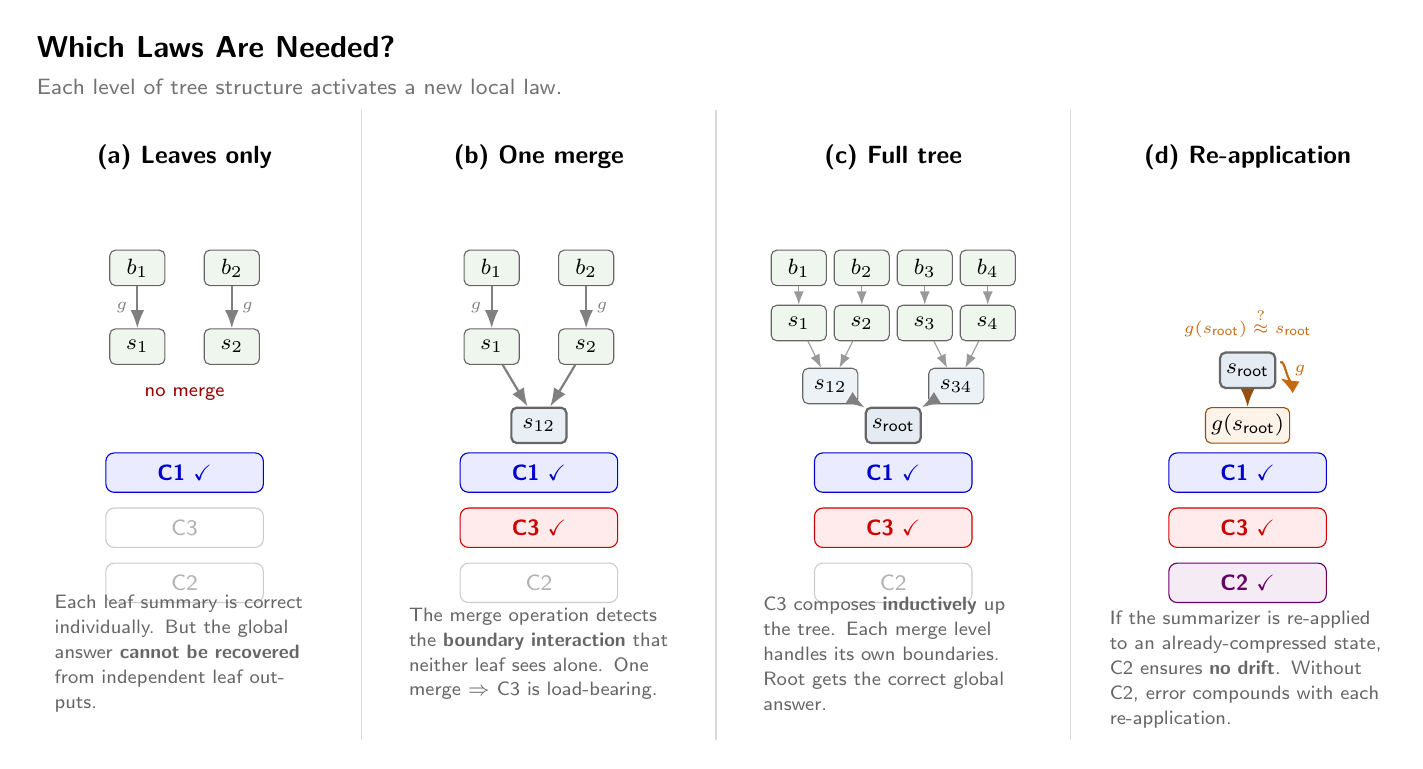
\begin{tikzpicture}[x=1cm,y=1cm,font=\sffamily,>=Latex]

  % Title
  \node[anchor=west, font=\sffamily\bfseries\fontsize{11}{13}\selectfont] at (0, 7.6)
    {Which Laws Are Needed?};
  \node[anchor=west, font=\sffamily\fontsize{8}{9.5}\selectfont, text=black!55] at (0, 7.1)
    {Each level of tree structure activates a new local law.};

  % Column positions
  \def\colA{2.0}
  \def\colB{6.5}
  \def\colC{11.0}
  \def\colD{15.5}

  % === Column 1: Zero merges (leaves only) ===
  \node[scenelabel] at (\colA, 6.2) {(a) Leaves only};

  % Mini tree: just leaves
  \node[treenode, fill=leafgreen!10] (a1) at (\colA-0.6, 4.8) {\footnotesize $b_1$};
  \node[treenode, fill=leafgreen!10] (a2) at (\colA+0.6, 4.8) {\footnotesize $b_2$};

  % Arrow down to summary
  \node[treenode, fill=leafgreen!10] (as1) at (\colA-0.6, 3.8) {\footnotesize $s_1$};
  \node[treenode, fill=leafgreen!10] (as2) at (\colA+0.6, 3.8) {\footnotesize $s_2$};
  \draw[->, black!50, thick] (a1) -- node[left, font=\sffamily\fontsize{6}{7}\selectfont] {$g$} (as1);
  \draw[->, black!50, thick] (a2) -- node[right, font=\sffamily\fontsize{6}{7}\selectfont] {$g$} (as2);

  % No connection between s1 and s2
  \node[font=\sffamily\fontsize{7}{8.5}\selectfont, text=red!60!black] at (\colA, 3.2) {no merge};

  % Law badges
  \node[activelaw=blue] at (\colA, 2.2) {C1 \checkmark};
  \node[inactivelaw] at (\colA, 1.5) {C3};
  \node[inactivelaw] at (\colA, 0.8) {C2};

  % Description
  \node[scenedesc] at (\colA, -0.1)
    {Each leaf summary is correct individually.
     But the global answer \textbf{cannot be recovered} from
     independent leaf outputs.};

  % === Column 2: One merge (2-leaf tree) ===
  \node[scenelabel] at (\colB, 6.2) {(b) One merge};

  \node[treenode, fill=leafgreen!10] (b1) at (\colB-0.6, 4.8) {\footnotesize $b_1$};
  \node[treenode, fill=leafgreen!10] (b2) at (\colB+0.6, 4.8) {\footnotesize $b_2$};
  \node[treenode, fill=leafgreen!10] (bs1) at (\colB-0.6, 3.8) {\footnotesize $s_1$};
  \node[treenode, fill=leafgreen!10] (bs2) at (\colB+0.6, 3.8) {\footnotesize $s_2$};
  \draw[->, black!50, thick] (b1) -- node[left, font=\sffamily\fontsize{6}{7}\selectfont] {$g$} (bs1);
  \draw[->, black!50, thick] (b2) -- node[right, font=\sffamily\fontsize{6}{7}\selectfont] {$g$} (bs2);

  % Merge node
  \node[treenode, fill=regCalm!12, line width=0.8pt] (bm) at (\colB, 2.8) {\footnotesize $s_{12}$};
  \draw[->, black!50, thick] (bs1) -- (bm);
  \draw[->, black!50, thick] (bs2) -- (bm);

  % Law badges
  \node[activelaw=blue] at (\colB, 2.2) {C1 \checkmark};
  \node[activelaw=red] at (\colB, 1.5) {C3 \checkmark};
  \node[inactivelaw] at (\colB, 0.8) {C2};

  \node[scenedesc] at (\colB, -0.1)
    {The merge operation detects the \textbf{boundary interaction}
     that neither leaf sees alone.
     One merge $\Rightarrow$ C3 is load-bearing.};

  % === Column 3: Full tree (multiple merges) ===
  \node[scenelabel] at (\colC, 6.2) {(c) Full tree};

  \node[treenode, fill=leafgreen!10] (c1) at (\colC-1.2, 4.8) {\footnotesize $b_1$};
  \node[treenode, fill=leafgreen!10] (c2) at (\colC-0.4, 4.8) {\footnotesize $b_2$};
  \node[treenode, fill=leafgreen!10] (c3) at (\colC+0.4, 4.8) {\footnotesize $b_3$};
  \node[treenode, fill=leafgreen!10] (c4) at (\colC+1.2, 4.8) {\footnotesize $b_4$};
  \node[treenode, fill=leafgreen!10] (cs1) at (\colC-1.2, 4.1) {\footnotesize $s_1$};
  \node[treenode, fill=leafgreen!10] (cs2) at (\colC-0.4, 4.1) {\footnotesize $s_2$};
  \node[treenode, fill=leafgreen!10] (cs3) at (\colC+0.4, 4.1) {\footnotesize $s_3$};
  \node[treenode, fill=leafgreen!10] (cs4) at (\colC+1.2, 4.1) {\footnotesize $s_4$};
  \draw[->, black!40] (c1) -- (cs1);
  \draw[->, black!40] (c2) -- (cs2);
  \draw[->, black!40] (c3) -- (cs3);
  \draw[->, black!40] (c4) -- (cs4);

  \node[treenode, fill=regCalm!10] (cm12) at (\colC-0.8, 3.3) {\footnotesize $s_{12}$};
  \node[treenode, fill=regCalm!10] (cm34) at (\colC+0.8, 3.3) {\footnotesize $s_{34}$};
  \draw[->, black!40] (cs1) -- (cm12);
  \draw[->, black!40] (cs2) -- (cm12);
  \draw[->, black!40] (cs3) -- (cm34);
  \draw[->, black!40] (cs4) -- (cm34);

  \node[treenode, fill=regCalm!15, line width=0.8pt] (croot) at (\colC, 2.8) {\footnotesize $s_\text{root}$};
  \draw[->, black!50, thick] (cm12) -- (croot);
  \draw[->, black!50, thick] (cm34) -- (croot);

  % Law badges
  \node[activelaw=blue] at (\colC, 2.2) {C1 \checkmark};
  \node[activelaw=red] at (\colC, 1.5) {C3 \checkmark};
  \node[inactivelaw] at (\colC, 0.8) {C2};

  \node[scenedesc] at (\colC, -0.1)
    {C3 composes \textbf{inductively} up the tree.
     Each merge level handles its own boundaries.
     Root gets the correct global answer.};

  % === Column 4: Re-application (multi-round) ===
  \node[scenelabel] at (\colD, 6.2) {(d) Re-application};

  % Same tree but with re-summarize arrow
  \node[treenode, fill=regCalm!15, line width=0.8pt] (droot) at (\colD, 3.5) {\footnotesize $s_\text{root}$};

  % Re-apply arrow (loop)
  \draw[->, thick, regSpike!80!black]
    ($(droot.east) + (0.05, 0.1)$) to[out=30,in=-30]
    node[right, font=\sffamily\fontsize{6.5}{8}\selectfont, text=regSpike!80!black] {$g$}
    ($(droot.east) + (0.05, -0.1)$);

  % Result
  \node[treenode, fill=regSpike!10, draw=regSpike!60!black] (droot2) at (\colD, 2.8)
    {\footnotesize $g(s_\text{root})$};
  \draw[->, thick, regSpike!60!black] (droot) -- (droot2);

  % Comparator
  \node[font=\sffamily\fontsize{6.5}{8}\selectfont, text=regSpike!80!black] at (\colD, 4.1)
    {$g(s_\text{root}) \stackrel{?}{\approx} s_\text{root}$};

  % Law badges
  \node[activelaw=blue] at (\colD, 2.2) {C1 \checkmark};
  \node[activelaw=red] at (\colD, 1.5) {C3 \checkmark};
  \node[activelaw=violet] at (\colD, 0.8) {C2 \checkmark};

  \node[scenedesc, text width=3.5cm] at (\colD, -0.3)
    {If the summarizer is re-applied to an already-compressed state,
     C2 ensures \textbf{no drift}.
     Without C2, error compounds with each re-application.};

  % === Dividers ===
  \foreach \x in {4.25, 8.75, 13.25} {
    \draw[black!15, line width=0.5pt] (\x, -1.2) -- (\x, 6.8);
  }

\end{tikzpicture}
\end{document}
